\chapter{Introduction --- orthography}
\label{cha:intr-orth}

In Part~\ref{part:phonology-phonetics}, I argued that \lT\ and \xD\ were phonologically distinct at least until and including the period when the Poets of the Princes were active. In this Part, I will argue that this phonological distinction had its impact on the orthography of lenition well into the Middle Welsh period. More specifically, I will demonstrate that word-initial lenition of \mw[]{p, t, c} was not written until about 1300%
\footnote{I consider \mw[]{k} an allograph of \mw[]{c} for the purpose of lenition, so obviously lenition of \mw[]{k} was not written either.}.
Thus, there existed a time from the Old Welsh period up until this point when lenition of  voiceless stops was not written word-initially, even though leniton of most other consonants was.

Orthographical representation of lenition arose at the end of the \gls{ow} period. At this time time, the distinction between \lT\ and \xD\ was still maintained. As a result, scribes trying to represent the existence of three different stop series (\xT, \lT, and \xD) were in trouble, because the Latin alphabet  provides not three but two sets of stop consonants. This made them unable to keep apart in writing all three stop series that Welsh had at the time%
\footnote{Similar trouble existed for fricatives, cf.\ \textcite[28]{russell_rowynniauc_2003}, who states that `[i]t has long been observed that, because of the rise of fricatives and spirants within the history of British, early Welsh was seriously understocked in signs to represent the full consonantal inventory.'}.

Word-initially, there was no natural association between \lT\ and \xD\ until the point when they merged phonologically, so the natural result of this phonology and the limitations of the Latin alphabet was to write lenited voiceless stops with \mw[]{p, t, c}. Thus, Early \gls{mw} orthography represented lenition only for consonants other than voiceless stops\footnote{Of course, lenition was not written for \mw{d} and \mw{rh} either, but orthographical representation for those consonants only became standard by the end of the \gls{mw} period.}.

\section{Some textual evidence}
\label{sec:two-exampl-mowm}
One manuscript illustrating this limited orthographical system of lenition is found in MS \gls{sA}, the Black Book of Chirk, which Example~\ref{ex:aylodeubrenyna} illustrates: 
\mwcc[ex:aylodeubrenyna]{\gls{sA}~4.9--10}{sef eu aylodeu e brenyn. \al{y u}eybyon ay neyeynt a\al{y k}euenderu.}{These are the members of the king: his sons and his nephews and his cousin.}
Here, lenition is represented following  \mw[his]{y} in \mw[sons]{ueybyon}, from unlenited \mw[]{meybyon}, but not in \mw[cousin]{keuenderu}, even though \mw{y} must obviously be translated as `his' before both words. In this example, the parallelism makes it obvious that \mw[]{keuenderu} should be lenited even though there is no orthographical lenition to back this up.

The fact that lenited \mw[]{p, t, c} are written exactly the same as their radical counterparts makes it difficult to identify the exact geographical and chronological extent to which the non-merger of \xD\ and \lT\ existed. The only way to identify this non-merger is usually by observing where in a \gls{mw} text we would expect lenition, but where it is not written. Naturally, these identifications require thorough knowledge on lenition in  the grammar of early \gls{mw}\footnote{I discuss my policy on where I may confidently expect lenition in Chapter~\ref{cha:some-phon-issu}.}. Fortunately, the early habit of not writing lenition of voiceless stops can be discerned even in the absence of such thorough knowledge in a few cases.

The basic fact that there was an early \gls{mw} period with orthographic lenition, with the exception of \lT, may be established even without knowledge of when exactly to expect lenition. This can be done on the basis of two manuscript copies of the elegy of Madog ap Maredudd. The opening lines of this poem as they are found in \gls{bbc}  and \gls{h}, respectively, are given in Example~\ref{ex:marwnadcomparison}.
\begin{mwl}
\item%
  \begin{minipage}[t]{0.45\textwidth}
    \mw{%
      Kẏwarchaw im ri.\ rad wobeith.\\
      Kẏwarchaw kẏwercheiſ e \al{c}anweith.\\
      Ẏ \al{p}rowi prẏdv.\ o\abbr{m} priwieth eurgert.\\
      ẏm argluit \al{k}edẏmteith.\\
      Ẏ \al{c}vinav madauc.\ metweith ẏ alar\\
      ae alon ẏm pop ieith.\\
      Doꝛ yſgoꝛ ẏſcvid \al{c}anhimteith.}\\
    (\acrshort{bbc}~52v.3--7)
  \end{minipage}~
  \begin{minipage}[t]{0.45\textwidth}
    \mw{%
      Kẏuarchaf ẏm ri rad o obeith.\\
      kẏuarchaf, kẏuercheis \al{g}anweith.\\
      ẏ \al{b}ꝛoui pꝛẏdu om pꝛifẏeith eurgert.\\
      ẏm arglwẏt \al{g}edymdeith.\\
      ẏ \al{G}wẏnaỽ madaỽc metueith.\ ẏ alar\\
      ae alon ẏm pob ẏeith\\
      Doꝛ ẏſgoꝛ ẏſgwẏd \al{g}anhẏmdeith.}\\
    (\acrshort{h}~47v.8--13)
  \end{minipage}
  \label{ex:marwnadcomparison}
\end{mwl}
Here, we see that lenition is written in \gls{bbc} to some extent, \eg in \mw[ mourning him]{ẏ alar}, but wherever lenition  of \mw[]{p, t, c} is written in \gls{h}, the radical is found in \gls{bbc}. These instances are marked. Note that non-word-initial lenition of voiceless stops does not necessarily differ between between \gls{bbc} and \gls{h}, \cf \mw[golden song]{eur\al{g}ert} in both manuscripts, but \mw[companion]{kedẏm\al{t}eith/gedym\al{d}eith}, so non-word-initial lenition was written differently from word-initial lenition by the time of \gls{bbc}\footnote{Part~\ref{part:orthography} primarily discusses morphophonemic word-initial lenition. Drawing the line between \gls{morphophonlen} and non-morphophonemic lenition (\gls{petr}) and between  word-initial lenition and non-word-initial lenition is a non-trivial task, which is discussed in Chapter~\ref{cha:some-phon-issu}.}.

Both manuscripts are datable. \Gls{bbc} dates from about 1250~\autocite[xxiv]{jones_rhagymadrodd_1982}, while \gls{h} dates from about 1300~\autocite{huws_llawysgrif_1981}. Additionally, the original composition of the poem is datable, because it mourns the death of a known person. It must thus have been written shortly after Madog ap Maredudd's death in 1160~\autocite[82]{jones_gwaith_1991}. Additionally, we know this poem was composedby Cynddelw Brydydd Mawr, who was active in the late twelfth century~\autocite[xxx]{jones_gwaith_1991}. From these dates we may conclude that lenition of \mw[]{p, t, c} was  not written by 1160, and this pattern was  not updated in \gls{bbc} around 1250, but in \gls{h} around 1300, lenition of voiceless stops could be written for all consonants.

Note that \gls{h}, while generally orthographically innovative, does show some traces of non-representation of lenition where a lenited voiceless stop undergoes provection, \ie a doubled \lT\ is consistently written with \mw[]{p, t, c}. An overview of such instances is given in Table~\ref{reasonlenitionexddt} in Chapter~\ref{cha:prov-mwbe-y} on provection in \mow[]{Beirdd y Tywysogion}.

Lenition is written in the \gls{bbc} recension of this poem in a handful of instances:
\begin{mwl}
  \mwc[ex:bbcdan]{\gls{bbc}~53r.4--5}{Llav eſcud. \al{dan} iſcud calchwreith.}{A quick hand under a vari-coloured shield.}
  \mwc[ex:bbcagar]{\gls{bbc}~53r.4 (margin)}{llawin gviar \al{a gar}.\ o kidweith.}{A bloody blade he loves, of joint battle.}
\end{mwl}
Here, Example~\ref{ex:bbcdan} contains an instance of \mw[under]{dan}, which is lenited because it is a reduced clitic. In Chapter~\ref{cha:some-phon-issu} I argue that such clitic reduction is not in fact lenition, and Chapter~\ref{cha:indep-comp-mwbr} demonstrates that these reduced clitics as well as instances of petrified lenition are represented with \mw[]{b, d, g} from an earlier date onwards than morphophonemically lenited voiceless stops. It is therefore no surprise that \mw[under]{dan} is written the way it is here. Example~\ref{ex:bbcagar} has \mw[loves]{a gar}, and is a genuine instance of morphophonemic lenition. It is written in the margin, which may point to a later insertion, but the insertion is written by the same hand, so it cannot have been much later. This one exception shows that scribes were aware of the possibility to represent lenited voiceless stops with \mw[]{b, d, g}, but that they chose not to do so\footnote{Section~\ref{sec:lenited-mwg} gives an insight into why scribes chose not to write lenition of \mw[]{p, t, c} despite being aware of the possibility.}. Isolated instances where lenition of \mw[]{p, t, c} are represented orthographically are found as early as the twelfth-century \mow[]{Braint Teilo}\footnote{Both translations are by \textcite[136]{davies_braint_1974}.}:
\begin{mwl}
  \mwc[ex:braintteiloardir]{\gls{bll} 63vb.1--2}{hac ap\abbr{er}ua ar \al{d}ir teiliau dẏr loggeu a diſcẏnno nẏthir.}{and harbourage on Teilo's land for the ships which may disembark on its land.}
%  \mwc[ex:braintteilodigauael]{\gls{bll} 63vb.14--15}{ẏ thir haẏ daẏr dẏ luẏd.\ dẏ uuner.\ di \al{g}auaẏl.}{Its lands (shall be) without military service, overlord, distraint.}
\end{mwl}
Here, \mw[on land]{ar dir}  presents a clear instance of word-initial morphophonemic lenition. Still, this instance merely  provides an exception to the rule, and it it took until the fourteenth century until lenited \mw[]{p, t, c} were represented as such in the orthography.

\section{Earlier scholarship}
\label{sec:earlier-literature}
Twentieth-century scholars mentioned that lenition is represented inconsistently, and some even noted that words beginning in specific consonants are often not lenited. However, none of these have problematised this issue.

\subsection{Evans}
\label{sec:evans}

\Textcite[\S 18]{evans_grammar_1964} notes that `[i]n MW orthography lenition is not regularly indicated.' He also notes the same for nasalisation, but not for spirantisation~\autocite[\S\S 24--25]{evans_grammar_1964}. This is unexpected: given how lenition is  more common and serves to disambiguate more meanings than either nasalisation or spirantisation, we would expect lenition to be the most frequently represented one of the three. Some examples of lenition given by Evans have counterexamples starting in voiceless stops. For example, \mw[Pwyll Prince of Dyfed]{Pwyll \al{P}endeuic Dyuet} is given as a counterexample to the rule that a noun in apposition to a personal name is lenited~\autocite[\S 19]{evans_grammar_1964}. However, this example may also precede orthographic lenition of voiceless stops, as it contains a text most likely composed some time before its earliest manuscript witness. Evans does attempt to find some amount of consistency in the inconsistency with which lenition is represented:
\tqt{A tenuis often remains unchanged after \mw[]{'th}: \mw[and thy sword]{a'th \al{c}ledeu} […], \mw[to thy castle]{y'th \al{c}astell}. […] Unvoicing of a media after a voiceless spirant is quite common in MW; note the following examples: \mw[thy body]{dy gorff \al{t}i} […], \mw[all the chains]{yr holl \al{k}adwyneu}.}{evans_grammar_1964}{\S 20N}
Evans may be quite right here that \mw[]{'th} and the other voiceless spirants may undo lenition of voiceless stops, but they may also simply be traces of an earlier, more general situation where lenition of voiceless stop was not written\footnote{Chapter~\ref{cha:welsh-laws} and Chapter~\ref{cha:stemm-mwbuch-dewi} give a more detailed discussion of how the orthography of an early text may leave traces in later manuscripts.}.

\subsection{Roberts}
\label{sec:roberts}

The prefaces of textual editions typically give an overview of the orthography used in these texts. The \gls{ll1} manuscript, containing \mw[]{Brut y Brenhinedd}, forms the basis of an edition
by \textcite{roberts_brut_1971}, which I will take as an example. The orthography of lenition in this manuscript is analysed in Chapter~\ref{cha:indep-comp-mwbr}, and it is just like the Black Book of Carmarthen in that lenition of \mw[]{p, t, c} is not represented. Roberts notes the following on the
orthography of stops and on lenition, respectively:
\tqt{Initially [b, d, g] are always denoted by \textit{b, d, g} ;
  medially they are usually represented by \textit{b, d, g}, with some
  examples of \textit{-p-, -t-, -k-}. Finally, [d] is always
  represented by \textit{t}, [g] by \textit{c} with the exception
  of \textit{og}, but final [b] is represented sometimes
  by \textit{p}, and sometimes by \textit{b, pob, pab, escyb}.  The
  unvoiced stops [p, t, k] occur initially and are written \textit{p,
    t, c/k}. \textit{c-} does not occur often and the scribe prefers
  to use \textit{k-}.  The convention of using \textit{k}
  with \textit{y, i,} or \textit{e} and \textit{c} with other vowels
  and consonants […] does not seem to have been followed and the
  same word may appear with initial \textit{c-} or \textit{k-}.
  As \textit{b, d, g} medially denote [b, d, g] the corresponding
  unvoiced stops can be written \textit{p, t, tt, k, kc}.
}{roberts_brut_1971}{xli}
There is no mention of how lenition is written under the discussion of the orthography of stops. Roberts, like Evans, observes that lenition is represented irregularly, and that this is unlike the spirant and nasal mutations. 
\tqt{Lenition of initial consonants is not always shown in the text
  but the scribe almost invariably denotes the spirant and nasal
  mutations }{roberts_brut_1971}{xlii}
He similarly does not mention how problematic this difference is. Not only did this generation of scholars fail to find a pattern in when lenition was and was not represented, but they also failed to see the need to find such a pattern at all, \ie they not only failed to find the solution to the topic of this thesis, but  even failed to find the topic at all.

\subsection{Haycock}
\label{sec:haycock}

Haycock, in her edition of the legendary poems in the Book of Taliesin goes a bit further and notices the following: `Lenition of initial p, t (and d) are not generally realized'~\autocite[p.~7, n.~18]{haycock_legendary_2015}. This is to my knowledge the first instance where a previous author saw that representation of lenition depended on whether the initial consonant is a voiceless stop\footnote{Here, lenited \mw[]{c} was already written, but not \mw[]{p, t}. This pattern is found more generally in the late thirteenth century.}. She does not discuss this pattern any further, but \textcite{Sad_Linguistic18} does discuss the orthography of lenition in \gls{bt} further. He notes that scribe X86 was broadly uniform in this pattern, and that the difference in date or genre of the texts copied by this scribe do little to change this uniformity~\autocite[164]{Sad_Linguistic18}. Table~\ref{tab:behaviourx86} shows that it is actually the a feature of the scribe's orthography to represent lenited \mw[]{c}, but not to write lenition of \mw[]{p, t}\footnote{The numbers given in this table are taken from samples from each of the manuscripts. For \acrshort{cca14}, ff.~33r--35v were taken; for \gls{sV}, ff.~1r--8v were taken. Both of these manuscripts contain recensions of \mw[]{Llyfr Cyfnerth}. For \acrshort{bt}, \mw[]{Armes Prydein}~\autocite{williams_armes_1972}, texts I–VI, XI–XII from \textcite{williams_canu_1960}, and texts 1–6, 9–10 from \textcite{haycock_prophecies_2013} were taken. From \acrshort{p6} pp.~17–20 were taken, which contain the text \mw[]{Gereint ac Enid}. }.
\begin{table}[h]
  \centering
  \begin{tabular}{lddddddd}
    \toprule
    \tch{MS} & \tch{\mw{b}} & \tch{\mw{g}} & \tch{\mw{ll}} & \tch{\mw{m}} & \tch{\mw{p}} & \tch{\mw{t}} & \tch{\mw{c}} \\
    \midrule
    \acrshort{cca14} & 92.3 & 100.0 & 100.0 & 85.7 & 14.3 & 0.0 & 95.8 \\
    \gls{sV} & 90.6 & 97.8 & 92.9 & 93.3 & 31.4 & 0.0 & 94.1 \\
    \acrshort{bt} & 91.4 & 80.8 & 92.5 & 85.7 & 33.3 & 11.5 & 78.0 \\
    \acrshort{p6} & 100.0 & 93.0 & 100.0 & 100.0 & 10.0 & 0.0 & 90.9 \\
    \bottomrule
  \end{tabular}%
  \caption{Percentual representation of lenition of voiceless stops in various manuscripts found in the hand of X86 (excluding research exceptions).}
  \label{tab:behaviourx86}
\end{table}

Table~\ref{tab:behaviourx86} shows that scribe X86 typically wrote lenition of consonants other than \mw[]{p, t}. However, the texts analysed here are copies rather than original texts. This makes it possible that this orthography was a feature of his exemplars. However, \acrshort{bt} contains compelling arguments that it was indeed X86 who added lenition of \mw[]{c}. The following line is found at the end of page~64:
\mwcc[llt6465]{\gls{bt} 64.26}{nyt ameſcut ygaỽ y gywlat/kywlat}{Not slow to pin an enemy down. \autocite[trans.][92]{clancy_triumph_1998}}
Here, \mw[enemy]{gywlat} is found below line 26, the last line of the page according to \textcite{evans_facsimile_1915}. The first word of the next page is \mw{kywlat}. A photograph of the relevant area is found in Figure~\ref{fig:p64}. In this photograph, \mw{gywlat} may not be made out, but investigation of the original under ultraviolet light revealed that the top half of these letters are still faintly discernible. A horizontal stroke in the first letter of the word must have marked the top of the \mw{g}, and cannot have marked a \mw{k}.  

\begin{figure}[h]
    \centering
    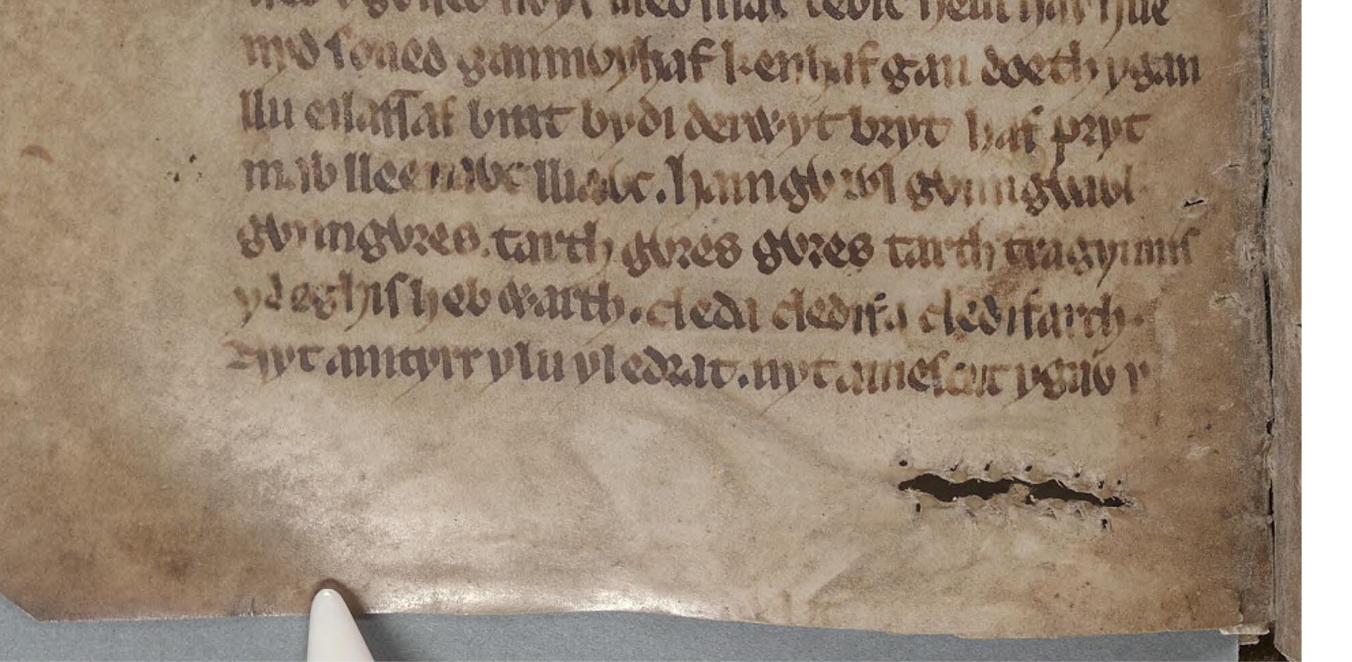
\includegraphics[width=\textwidth]{3orth/images/canvas.png}
    \caption[The bottom of \gls{bt} p.~64]{The bottom of \gls{bt} p.~64. Image credit: The National Library of Wales}
    \label{fig:p64}
\end{figure}

The easiest way to account for this situation is that scribe X86  copied the word \mw{kywlat} twice: first he wrote it as a catchword to make sure the quire starting with page 65 would be placed immediately following the quire ending with page 64. The second time it is found as the first word of page 65. In the first instance, he adds orthographic representation of lenition, and in the second he copies his exemplar directly. The reason he did not add lenition in the second instance is most likely due to him forgetting about the syntactic context of this word by the time he had his next quire before him. This instance singularly tells us that it was scribe X86 was the one who added orthographic lenition to his texts, and that his exemplar did not have lenition represented orthographically.


\subsection{Sims-Williams}
\label{sec:sims-williams}

\Textcite[107n]{Sim_Buchedd18} notes that `[s]ometimes the radical is written even when lenition is required grammatically, \eg \mw[his patrimony]{y \al{t}reftat ef}; \mw[from exhaustion]{o \al{t}rablinder}; \mw[from this kingdom]{o'r \al{t}eyrnnas honn}.' The bare fact that lenition is sometimes not written is noticed here, and all his examples start with \mw[]{t}, yet there is no remark that non-lenition may be conditioned by the initial consonant. I found that lenition is not represented 12 times in \mw[]{Buchedd Beuno}, and every single one of these instances starts with \mw[]{t}. This implies that there was a period or an area where lenition of \mw[]{p, c} was written but not \mw[]{t}\footnote{I have been unable to confirm the existence of such a phase in Chapter~\ref{cha:indep-comp-mwbr}, but manuscripts \gls{sB}\gls{sE} in Chapter~\ref{cha:welsh-laws} show quite a bit more non-lenition of \mw[]{t} than of \mw[]{p}, but the pattern is muddied by the fact that these manuscripts have complicated textual histories.}.

However, lenition of \mw[]{t} is represented more frequently than it is not. Another saint's life found in the same manuscript  is discussed in Chapter~\ref{cha:stemm-mwbuch-dewi} as \gls{j119}. Here, it is concluded that orthographical lenition of \mw[]{c} was found in the original Welsh composition because it is represented consistently, while lenited \mw[]{p, t} are represented inconsistently, and were therefore added to the text at a later stage. This makes it difficult to pinpoint the time or place when only lenited \mw[]{t} was not represented, because \gls{j119} provides only a copy of a text which has this pattern, not the text itself.

\subsection{Van Sluis}
\label{sec:van-sluis}

Existential verb \oes\ and the verbal ending \ei\ are noticed by~\textcite{van_development14} as causing lenition to immediately following subjects and objects alike, but not to \mw[]{p, t, c}. This behaviour contrasts with other types of postverbal lenition, such as object lenition and \gls{np} lenition. This pattern is observed in some of the earliest Mabinogion texts, \ie \mow{Culhwch ac Olwen} and \mow{Pwyll Pendefig Dyfed}. These texts are found in the \gls{wbr}, which dates from the mid-fourteenth century, but are thought to have been composed earlier\footnote{\Textcite[43]{rodway_date_2005} dates the composition of \mow[]{Culhwch ac Olwen} to the second half of the twelfth century, but is unsure about \mow[]{Pwyll Pendefic Dyfed}~\autocite[59]{Rod_Where07}. The \gls{wbr} dates to the mid-fourteenth century~\autocite[59]{huws_medieval_2000}.}.

Because non-lenition of \mw{p, t, c} is found following postverbal contact lenition, but not following object lenition or \gls{np} lenition, \textcite{van_development14} considers this non-lenition a specific feature of \ei\ and \oes\ only. In light of the difference in orthography between \gls{bbc} and \gls{h}, however, it may make more sense to think of non-lenition of \mw[]{p, t, c} following \ei\ and \oes\ as an older orthographical stratum, and to think of object and \gls{np} lenition as later innovations to the text\footnote{In fact, \textcite{van_development14} describes how object lenition and \gls{np} lenition gained ground in the \gls{mw} period. Chapter~\ref{cha:welsh-laws} explores how older orthographical strata may be transmitted in later \gls{mw}.}.

\section{Stop orthography as a dating criterion}
\label{sec:lenit-voic-stops-1}
Any student of Welsh quickly learns to recognise the difference between \gls{ow}, \gls{mw} and \gls{mow} based on where lenition is represented. \Gls{ow} has no orthographic lenition even though we know it existed in the spoken language, while \gls{mw} does have orthographic lenition, except for \mw{d, rh}. \Gls{mow} has orthographic lenition for all consonants that lenite phonologically, including \mow[]{d, rh}. Thus, a student will easily be able to identify just on the basis of where lenition is represented whether any text before him dates from the \gls{ow} period (9th--11th centuries), the \gls{mw} period (12th--14th centuries), or the \gls{mow} period (15th century onwards)

I propose one more intermediate stage between \gls{ow} and \gls{mow}: in early \gls{mw}, lenition of voiceless stops was not represented orthographically word-initially, while in later \gls{mw} it was. Thus, early \gls{mw} texts may be recognised as such because they do not represent lenition of voiceless stops, and late \gls{mw} texts may be recognised as such because they do. This raises the question when these lenited voiceless stops came to be represented with \mw[]{b, d, g}. In a text where  lenition is represented orthographically, except for voiceless stops, we may postulate a \lat{terminus ante quem} as well as a \lat{terminus post quem} for its original composition: it must originally have been composed before lenition of voiceless stops was represented orthographically, and after lenition started being represented at all.

The more precisely the origin of orthographical lenition of voiceless stops may be pinpointed, the more precisely texts having or lacking this feature may be dated. This is one goal of Part~\ref{part:orthography}. Moreover, \textcite{van_development14} saw that some grammatical environments are particularly conservative in the sense that lack of orthographical lenition may carry over in newer texts. If these environments can be identified, then traces of  earlier orthographical strata in younger manuscripts may be found. This is another goal of Part~\ref{part:orthography}.

\section{Other dating criteria}
\label{sec:other-dating-crit}

It is helpful to compare this task with earlier efforts to date and localise \gls{mw} texts based on linguistic or orthographical criteria. Here, I discuss some of these efforts.

An example of a datable development in Medieval Welsh is the relative frequency of third person singular preterite indicative ending \mw[]{\mbox{-w(y)s}} and \mw[]{-awdd}. Here, \textcite{Rod_Datable98} sees a marked increase in the use of \mw[]{-awdd} in the work of thirteenth-century poets compared to their twelfth-century counterparts. Poetry from about 1300 has near-universal \mw[]{-awdd}. He also studied the relative frequency of these markers in prose, and they change in roughly the same period in prose as they did in poetry. \Textcite[68--71]{Rod_Two03} adds to this verbal ending the third person singular imperfect endings \mw[]{\mbox{-i}} and \ei, the former of which gradually fell out of use over the twelfth and early thirteenth centuries. Still, there was no period in which \mw[]{-i} was more common than \ei. Another such variable is the shift from third person singular present subjunctive \mw[]{\mbox{-wy/-oe}} towards \mw[]{-o}. Here, \textcite[71--73]{Rod_Two03} observes a dramatic rise of \mw[]{-o} in the first half of the thirteenth century, although the situation in poetry is somewhat different from prose. Ending \mw[]{-o} was consistently employed as early as the twelfth-century \mow{Braint Teilo}, and \textcite[73]{Rod_Two03} only found one occurrence of \mw[]{-wy} in prose in \mow[]{Culhwch ac Olwen}. \Textcite{Rod_Where07} provides an example of how the relative incidence of verbal endings may help in creating a rough chronology, and how this methodology compares to other methods in establishing the where and when of medieval literature. The most complete overview of which verbal endings are typical of which period is found in \textcite[166]{rodway_dating_2013}, which shows that compounding insights into the chronology of several developments allows one to date texts with a precision of roughly half a century.

Many of these developments described by Rodway occurred in the thirteenth century, and they thus seem to be roughly contemporaneous with the shift towards representing lenition of voiceless stops. Also, Rodway noticed how prose and poetry sometimes but not always undergo language change at differing moments, so textual genre may serve as a confounding variable\footnote{I have not found any consistently differing orthographies of lenition between poetry and prose. The difference between the orthography lenition and which verbal ending to use may lie in the fact that the former variable is mostly confined to orthography, while making changes in verbal endings changes poetry when it is spoken as well.}.

%% PSW is not too relevant after all

\Textcite{Tho_Middle93} proposes that linguistic criteria may be used not only for dating the composition of a text, but also for geographic identification. I will discuss two of his variables:  stem-formative yod which may be present or absent, \eg \mw[sureties]{meychyeu/meicheu}, and stem-formative \mw[]{-th-/-t-} in inflected forms of \mw[with]{gan} and \mw[between]{rwng}, \eg \mw[with him]{ganthaw/gantaw}\footnote{His third variable is third person singular \mw[]{-awd/-ws}, but \textcite{Rod_Datable98} later showed that variation here is chiefly chronological, not dialectal.}. Here, high incidence of yod is associated with northern texts, and low incidence with southern texts. For the inflected prepositions, stem-formative \mw[]{\mbox{-th-}} generally appears in northern texts, and \mw[]{\mbox{-t-}} appears in southern texts. Consequently, there is a strong positive correlation between these features: high frequency of yod implies high frequency of stem-formative \mw[]{\mbox{-th-}}. This research shows the value in considering multiple linguistic variables when establishing time and place of composition. If one wishes to establish the place of a text's composition, but the text is too short or lacking in sufficient tokens to judge its dialectal affiliation based on either variable, then one may use both variables to reach a reliable judgment.

The case of stem-formative yod is more complicated than described above, however. \Textcite{Rus_Celtic90}, for example, noted that variation between \mw[]{\mbox{-awc}} and \mw[]{\mbox{-yawc}} is  lexically conditioned to a great extent. This means that incidence of yod in a text does not correlate solely with its geographical origin, but also that some words or morphemes are more likely to contain a yod than others. \Textcite[106]{Wil_Lexical05}  notes that some words show no variation at all, meaning that these items occur with or without yod in both northern and southern texts, and the items that do vary do so according to a pattern reminiscent of lexical diffusion of sound change\footnote{Lexical diffusion occurs when a modification is modified in a subset of a language's lexicon only, and then spreads gradually to other lexical items.}. \Textcite[116]{Wil_Lexical05} then lists fourteen lexical items that occur frequently and show variability regarding presence or absence of yod in his corpus of northern and southern law manuscripts. He notes that the relative frequency of yod has the following order, from low frequency of yod to high: \mw[relics]{kreir(y)eu} < \mw[pregnant]{beich(y)awc} < \mw[testimony]{tyst(y)olaeth} < \mw[lawful]{kyfreith(y)awl} < \mw[laws]{kyfreith(y)eu} < \mw[witnesses]{tyst(y)on} < \mw[already]{eiss(y)oes} < \mw[try]{keiss(y)aw} < \mw[bullock]{eid(y)on} = \mw[penny]{kein(y)awc} < \mw[sons]{meib(y)on} < \mw[priest]{effeir(y)at} < \mw[eye-witnesses]{gwybyd(y)eit} < \mw[men]{dyn(y)on}. This order means \eg that \mw[]{kreir(y)eu} appears with yod in relatively fewer instances and in fewer manuscripts than \mw{beich(y)awc} does, et cetera. \Textcite[117]{Wil_Lexical05} moreover notes that there is agreement between the texts about the nature of the variation, meaning that one may somewhat confidently predict that a text using yodless \mw[]{meibon} will also use yodless \mw[]{tyston}, because the former item has yod appearing more frequently than the latter. The raw percentages given by \textcite{Tho_Middle93} do not reflect this complexity.

Willis's methodology and observations demonstrate the importance of comparing like with like. That is: one should compare manuscript texts that are as similar to each other as possible, except for the variable under study. Chapter~\ref{cha:indep-comp-mwbr} compares translations of the same text, and they chiefly differ in the date of their translation into \gls{mw}. Consequently, the different texts under comparison are similar in variables such as genre and vocabulary, but they represent diffent stages of the language. Willis's observations also teach us that the evidential value of a single form containing yod or not differs from word to word. In \mw[]{kreir(y)eu}, for example, yod is quite rare across manuscripts, so a manuscript writing yod is strong evidence for a northern affiliation. Conversely, yodless \mw[]{kreireu} is a more trivial find, so it is not as strong an indicator of southern affiliation. The reverse is the case with \mw[]{effeir(y)at}, where yod is found in a high percentage of instances, and a majority of manuscripts have yod. Therefore, absence of yod in this word is strongly indicative of a southern affiliation, while its presence is rather trivial. Chapter~\ref{cha:stemm-mwbuch-dewi} discusses how manuscripts may share representation of lenition, or they may share lack of representation. Both types of  instances may be used to argue for a close stemmatic relationship, but the evidential value of represented lenition or lack thereof depends on the grammatical environment which causes lenition, just like the evidential value of stem-formative yod in establishing dialectal affiliation depends on the word in question.

\section{Overview}
\label{sec:overview}

This section presents an overview of the chapters in Part~\ref{part:orthography}, and how they  cumulatively build understanding of how lenited voiceless stops developed orthographically.

Chapter~\ref{cha:some-phon-issu} primarily treats some methodological issues. Firstly, it establishes that a phonological contrast between \lT\ and \xD\ only existed word-initially. And thus only word-initially is there a development to be studied. Hence, only word-initial lenition is considered, and not word-medial or word final lenition. This, of course, requires a definition for `word'. It is found that a universal definition of `word' is not available, and is perhaps even impossible. Still, a working definition is reached for this thesis. Primary data in Part~\ref{part:orthography} comprises mostly instances where lenition is and is not represented in various \gls{mw} texts. This requires a working definition of lenition, which is reached in this chapter. Finally, counting instances where lenition is not written implies exhaustive knowledge of rules governing \gls{mw} lenition. In order to accomplish this, I discuss all the environments which are found to cause lenition, and I discuss where non-orthographic lenition is held to exist even though it cannot be seen.

Chapter~\ref{cha:indep-comp-mwbr} serves to establish a chronology of the developments based on independent translations of Geoffrey of Monmouth's \lat{Historia Regum Brittanniae}. These translations give various snapshots of different stages of thirteenth-century and fourteenth-century Welsh. Here, three orthographical stages may be discerned. Up until the mid-thirteenth century, lenited \mw[]{p, t, c} were not represented; in the late thirteenth century, lenited \mw[]{c} was represented, but not \mw[]{p, t}; in the fourteenth century, all three consonants had lenition represented. These results may be used to date the original composition of hitherto undated texts.

Chapter~\ref{cha:welsh-laws} discusses the orthography of several law manuscripts containing \mow[]{Llyfr Iorwerth}. Here, the goal is to chart how an original composition predating the thirteenth century undergoes changes as it is copied into the thirteenth century and onwards. It is found that even some of the more innovative scribes from the fourteenth century preserve traces of older orthography, thus creating a textual form distinguishable from compositions contemporary with these scribes. Moreover, the chapter explores some alternative ways in which scribes modernised lack of orthographic lenition beyond simply filling in lenition where there was an unlenited consonant before. Finally, it gives indicators how comparing lenition in different manuscripts may be used to argue for a particular stemmatic relationship, which Chapter~\ref{cha:stemm-mwbuch-dewi} then builds on.

Chapter~\ref{cha:stemm-mwbuch-dewi} takes three manuscript witnesses of \mow[]{Buchedd Dewi}, and explores how correspondences or lack thereof in the orthography of lenition may be used to create a stemma of the various manuscript witnesses, and it even allows for the dating of hypothesised nodes in this stemma. 


%%% Local Variables:
%%% mode: latex
%%% TeX-master: "../main"
%%% coding: utf-8
%%% End:
